\section{Decodificador 2 a 4 \label{sec:s3}}

\begin{center}
	\begin{minipage}{12cm}
		\begin{tcolorbox}[title=Actividad 3]
			Completar el código del decodificador 2 a 4 en el lenguaje de su elección. Compilar y simular.  Configurar en la tarjeta DE2-115, asignar interruptores como entradas y LED´s para observar la salida.
		\end{tcolorbox}	
	\end{minipage}
\end{center}

La visualización RTL del decodificador 2 a 4 en Verilog se muestra en la \autoref{fig:decoder_2_4_rtl}. Como se observa, la implementación del decodificador 2 a 4 se hace utilizando una instancia de decodificador. Las simulaciones para el código en Verilog se visualizan en la \autoref{fig:decoder_2_4_WaveBi} en base binaria y en la \autoref{fig:decoder_2_4_WaveDe} en base decimal. Se utilizaron todos los valores posibles en las entradas para observar un comportamiento completo en la salida.

\begin{figure}[ht]
	\centering
	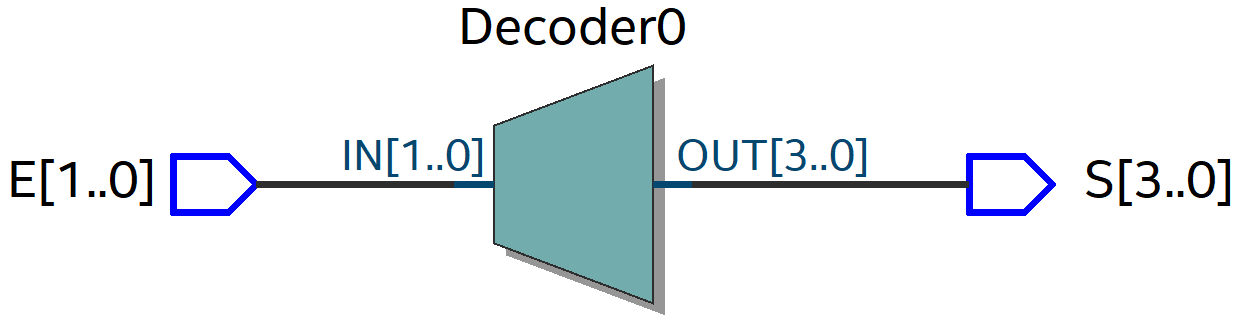
\includegraphics[scale=0.5]{Decoder_2_4_RTL.png}
	\caption{Diagrama RTL del decodificador 2 a 4. \label{fig:decoder_2_4_rtl}}
\end{figure}

\begin{figure}[ht]
	\centering
	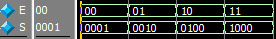
\includegraphics[scale=1.5]{Decoder_2_4_WaveBi.png}
	\caption{Simulación del decodificador 2 a 4 con el visor de formas de onda de ModelSim (Base binaria). \label{fig:decoder_2_4_WaveBi}}
\end{figure}

\begin{figure}[ht]
	\centering
	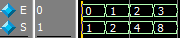
\includegraphics[scale=2]{Decoder_2_4_WaveDe.png}
	\caption{Simulación del decodificador 2 a 4 con el visor de formas de onda de ModelSim (Base decimal). \label{fig:decoder_2_4_WaveDe}}
\end{figure}